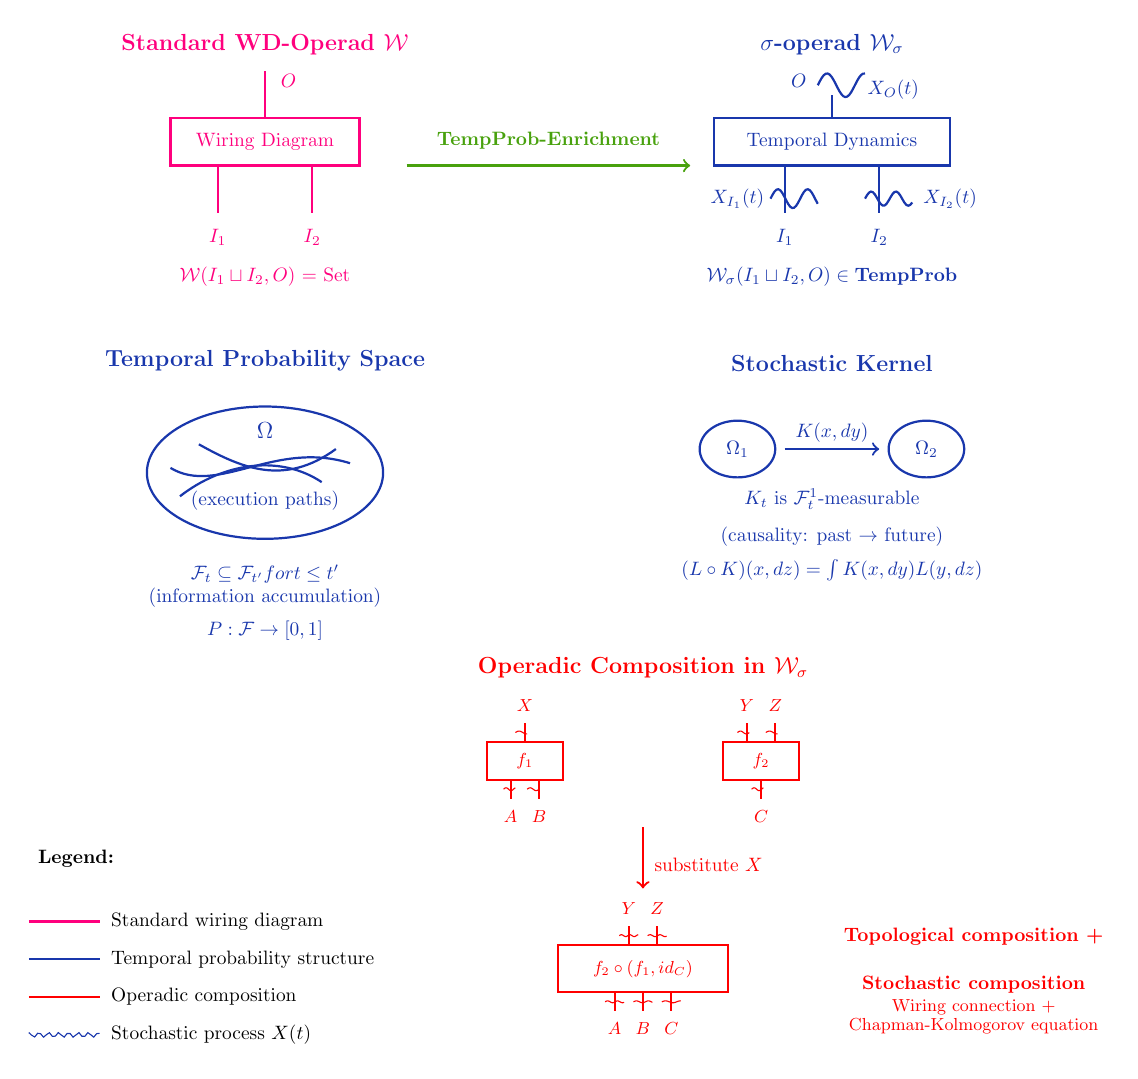
\begin{tikzpicture}[scale=0.6, every node/.style={scale=0.7}]

% Define colors - High Contrast Professional Palette
\definecolor{wdcolor}{RGB}{255, 0, 125}
\definecolor{tempcolor}{RGB}{25, 55, 172}
\definecolor{enrichcolor}{RGB}{72, 161, 13}
\definecolor{compcolor}{RGB}{255, 0, 0}

% Title
% \node[above] at (0, 8) {\Large\textbf{$\sigma$-operads: TempProb-Enriched Wiring Diagrams}};

% Part 1: Standard Wiring Diagram (left side)
\begin{scope}[shift={(-6, 4)}]
    \node[above, wdcolor, font=\large] at (0, 2.2) {\textbf{Standard WD-Operad $\mathcal{W}$}};

    % Input interfaces
    \draw[thick, wdcolor] (-1, -1) -- (-1, 0);
    \draw[thick, wdcolor] (1, -1) -- (1, 0);
    \node[below, wdcolor] at (-1, -1.2) {$I_1$};
    \node[below, wdcolor] at (1, -1.2) {$I_2$};

    % Box
    \draw[thick, wdcolor] (-2, 0) rectangle (2, 1);
    \node[wdcolor] at (0, 0.5) {Wiring Diagram};

    % Output interface
    \draw[thick, wdcolor] (0, 1) -- (0, 2);
    \node[above, wdcolor] at (0.5, 1.5) {$O$};

    % Hom-set notation
    \node[below, wdcolor] at (0, -2) {$\mathcal{W}(I_1 \sqcup I_2, O)$ = Set};
\end{scope}

% Arrow indicating enrichment
\draw[->, thick, enrichcolor] (-3, 4) -- (3, 4);
\node[above, enrichcolor] at (0, 4.2) {\textbf{TempProb-Enrichment}};

% Part 2: Temporal Probability Enriched (right side)
\begin{scope}[shift={(6, 4)}]
    \node[above, tempcolor, font=\large] at (0, 2.2) {\textbf{$\sigma$-operad $\mathcal{W}_\sigma$}};

    % Input interfaces with temporal processes
    \draw[thick, tempcolor] (-1, -1) -- (-1, 0);
    \draw[thick, tempcolor] (1, -1) -- (1, 0);
    \node[below, tempcolor] at (-1, -1.2) {$I_1$};
    \node[below, tempcolor] at (1, -1.2) {$I_2$};

    % Temporal processes at inputs
    \draw[tempcolor, thick, domain=0:1] plot (\x-1.3, {0.2*sin(10*\x r) - 0.7});
    \draw[tempcolor, thick, domain=0:1] plot (\x+0.7, {0.15*sin(12*\x r) - 0.7});
    \node[tempcolor] at (-2, -0.7) {$X_{I_1}(t)$};
    \node[tempcolor] at (2.5, -0.7) {$X_{I_2}(t)$};

    % Box with temporal dynamics
    \draw[thick, tempcolor] (-2.5, 0) rectangle (2.5, 1);
    \node[tempcolor] at (0, 0.5) {Temporal Dynamics};

    % Output with temporal process
    \draw[thick, tempcolor] (0, 1) -- (0, 1.5);
    \node[above, tempcolor] at (-0.7, 1.5) {$O$};
    \draw[tempcolor, thick, domain=0:1] plot (\x-0.3, {0.25*sin(8*\x r) + 1.7});
    \node[tempcolor] at (1.3, 1.6) {$X_O(t)$};

    % Hom-object notation
    \node[below, tempcolor] at (0, -2) {$\mathcal{W}_\sigma(I_1 \sqcup I_2, O) \in \mathbf{TempProb}$};
\end{scope}

% Part 3: Temporal Probability Space Details (middle-left)
\begin{scope}[shift={(-6, -2.5)}]
    \node[above, tempcolor, font=\large] at (0, 2) {\textbf{Temporal Probability Space}};

    % Sample space
    \draw[thick, tempcolor] (0, 0) ellipse (2.5 and 1.4);
    \node[tempcolor, font=\large] at (0, 0.9) {$\Omega$};
    \node[tempcolor] at (0, -0.6) {(execution paths)};

    % Trajectories
    \draw[tempcolor, thick] (-1.8, -0.5) .. controls (-0.9, 0.2) and (0.3, 0.4) .. (1.2, -0.2);
    \draw[tempcolor, thick] (-1.4, 0.6) .. controls (-0.5, 0.1) and (0.4, -0.3) .. (1.5, 0.5);
    \draw[tempcolor, thick] (-2.0, 0.1) .. controls (-1.0, -0.5) and (0.2, 0.7) .. (1.8, 0.2);

    % Filtration
    \node[below, tempcolor] at (0, -1.8) {$\mathcal{F}_t \subseteq \mathcal{F}_{t'} \text{ for } t \leq t'$};
    \node[below, tempcolor] at (0, -2.3) {(information accumulation)};

    % Measure
    \node[below, tempcolor] at (0, -3) {$\mathbb{P}: \mathcal{F} \to [0,1]$};
\end{scope}

% Part 4: Stochastic Kernel (middle-right)
\begin{scope}[shift={(6, -2.5)}]
    \node[above, tempcolor, font=\large] at (0, 2) {\textbf{Stochastic Kernel}};

    % Source space
    \draw[thick, tempcolor] (-2, 0.5) ellipse (0.8 and 0.6);
    \node[tempcolor] at (-2, 0.5) {$\Omega_1$};

    % Target space
    \draw[thick, tempcolor] (2, 0.5) ellipse (0.8 and 0.6);
    \node[tempcolor] at (2, 0.5) {$\Omega_2$};

    % Kernel arrow
    \draw[->, thick, tempcolor] (-1, 0.5) -- (1, 0.5);
    \node[above, tempcolor] at (0, 0.5) {$K(x, dy)$};

    % Adaptedness condition
    \node[below, tempcolor] at (0, -0.2) {$K_t$ is $\mathcal{F}_t^1$-measurable};
    \node[below, tempcolor] at (0, -1) {(causality: past $\to$ future)};

    % Chapman-Kolmogorov
    \node[below, tempcolor] at (0, -1.7) {$(L \circ K)(x, dz) = \int K(x, dy) L(y, dz)$};
\end{scope}

% Part 5: Composition Diagram (bottom)
\begin{scope}[shift={(2, -10)}]
    \node[above, compcolor, font=\large] at (0, 3) {\textbf{Operadic Composition in $\mathcal{W}_\sigma$}};

    % First component
    \begin{scope}[shift={(-2.5, 1)}]
        \draw[thick, compcolor] (-0.8, 0) rectangle (0.8, 0.8);
        \node[compcolor, font=\small] at (0, 0.4) {$f_1$};

        \draw[thick, compcolor] (-0.3, 0) -- (-0.3, -0.4);
        \draw[thick, compcolor] (0.3, 0) -- (0.3, -0.4);
        \node[below, compcolor, font=\small] at (-0.3, -0.5) {$A$};
        \node[below, compcolor, font=\small] at (0.3, -0.5) {$B$};

        \draw[thick, compcolor] (0, 0.8) -- (0, 1.2);
        \node[above, compcolor, font=\small] at (0, 1.3) {$X$};

        % Temporal processes (smaller)
        \draw[compcolor, domain=0:0.25] plot (\x-0.45, {0.03*sin(30*\x r) + -0.2});
        \draw[compcolor, domain=0:0.25] plot (\x+0.05, {0.03*sin(25*\x r) + -0.2});
        \draw[compcolor, domain=0:0.25] plot (\x-0.2, {0.03*sin(20*\x r) + 1.0});
    \end{scope}

    % Second component
    \begin{scope}[shift={(2.5, 1)}]
        \draw[thick, compcolor] (-0.8, 0) rectangle (0.8, 0.8);
        \node[compcolor, font=\small] at (0, 0.4) {$f_2$};

        \draw[thick, compcolor] (0, 0) -- (0, -0.4);
        \node[below, compcolor, font=\small] at (0, -0.5) {$C$};

        \draw[thick, compcolor] (-0.3, 0.8) -- (-0.3, 1.2);
        \draw[thick, compcolor] (0.3, 0.8) -- (0.3, 1.2);
        \node[above, compcolor, font=\small] at (-0.3, 1.3) {$Y$};
        \node[above, compcolor, font=\small] at (0.3, 1.3) {$Z$};

        % Temporal processes (smaller)
        \draw[compcolor, domain=0:0.25] plot (\x-0.2, {0.03*sin(30*\x r) + -0.2});
        \draw[compcolor, domain=0:0.25] plot (\x-0.5, {0.03*sin(25*\x r) + 1.0});
        \draw[compcolor, domain=0:0.25] plot (\x+0.1, {0.03*sin(20*\x r) + 1.0});
    \end{scope}

    % Composition arrow (Vertical now)
    \draw[->, thick, compcolor] (0, 0) -- (0, -1.3);
    \node[right, compcolor] at (0.1, -0.8) {substitute $X$};

    % Composed system
    \begin{scope}[shift={(0, -3.5)}]
        \draw[thick, compcolor] (-1.8, 0) rectangle (1.8, 1);
        \node[compcolor, font=\small] at (0, 0.5) {$f_2 \circ (f_1, \text{id}_C)$};

        % Inputs
        \draw[thick, compcolor] (-0.6, 0) -- (-0.6, -0.4);
        \draw[thick, compcolor] (0, 0) -- (0, -0.4);
        \draw[thick, compcolor] (0.6, 0) -- (0.6, -0.4);
        \node[below, compcolor, font=\small] at (-0.6, -0.5) {$A$};
        \node[below, compcolor, font=\small] at (0, -0.5) {$B$};
        \node[below, compcolor, font=\small] at (0.6, -0.5) {$C$};

        % Outputs
        \draw[thick, compcolor] (-0.3, 1) -- (-0.3, 1.4);
        \draw[thick, compcolor] (0.3, 1) -- (0.3, 1.4);
        \node[above, compcolor, font=\small] at (-0.3, 1.5) {$Y$};
        \node[above, compcolor, font=\small] at (0.3, 1.5) {$Z$};

        % Temporal processes (smaller and better positioned)
        \draw[compcolor, domain=0:0.4] plot (\x-0.8, {0.02*sin(30*\x r) + -0.2});
        \draw[compcolor, domain=0:0.4] plot (\x-0.2, {0.02*sin(25*\x r) + -0.2});
        \draw[compcolor, domain=0:0.4] plot (\x+0.4, {0.02*sin(20*\x r) + -0.2});
        \draw[compcolor, domain=0:0.4] plot (\x-0.5, {0.02*sin(35*\x r) + 1.2});
        \draw[compcolor, domain=0:0.4] plot (\x+0.1, {0.02*sin(30*\x r) + 1.2});
    \end{scope}

    % Explanation
    \node[below, compcolor] at (7, -2) {\textbf{Topological composition +}};
    \node[below, compcolor] at (7, -3) {\textbf{Stochastic composition}};
    \node[below, compcolor, font=\small] at (7, -3.5) {Wiring connection +};
    \node[below, compcolor, font=\small] at (7, -3.9) {Chapman-Kolmogorov equation};
\end{scope}

% Legend
\begin{scope}[shift={(-10, -12)}]
    \node[above] at (0, 1) {\textbf{Legend:}};

    \draw[thick, wdcolor] (-1, 0) -- (0.5, 0);
    \node[right] at (0.6, 0) {Standard wiring diagram};

    \draw[thick, tempcolor] (-1, -0.8) -- (0.5, -0.8);
    \node[right] at (0.6, -0.8) {Temporal probability structure};

    \draw[thick, compcolor] (-1, -1.6) -- (0.5, -1.6);
    \node[right] at (0.6, -1.6) {Operadic composition};

    \draw[tempcolor, domain=-1:0.5] plot (\x, {0.05*sin(30*\x r) + -2.4});
    \node[right] at (0.6, -2.4) {Stochastic process $X(t)$};
\end{scope}

\end{tikzpicture}
